\chapter{Introduction and Motivation}\label{ch:introduction}

Helicopters are a vital part of the transport of personnel to offshore installations along the Norwegian coast. Offshore personnel report fear of being involved in helicopter incidents. They also experience unease from flying in turbulent and bad weather (\cite{wasilewska2019}). These weather types may be causal to lightning incidents, as suggested in earlier work (e.g. \cite{lande1999}; \cite{wilkinson2013}; \cite{smart1997}). It has been estimated that the repair cost due to a lightning strike to a helicopter was on the order of 100,000 U.S. Dollars (\cite{lande1999}). The incident rate can be estimated from earlier data sets to about 2.05 per year for Norwegian operators in the period 1979-1999. This would then result in the accumulated economic loss of about 4 300 000 U.S. Dollars for the Norwegian operators. This potential in economic loss is severe in itself, but added onto this is also the danger helicopter pilots and passengers are put in, when the aircraft is hit by lightning. There are two major helicopter crashes related to lightning in the last 30 years (1995 and 2001) as discussed later in this section. By comparison, in the same period there has been only one airplane crash among the Norwegian operators (\cite{bodo}), even though airplanes are flying much more frequently in Norway. It is therefore imperative to exhaust the investigation into the causes of and possible ways to prevent helicopter related incidents. 

Lightning strikes can in various ways be the cause of helicopter incidents. These incidents include events when rotors have been destroyed, as in the case of Flight 56 in 1995 (\cite{smart1997}). Sometimes a breakdown of the structural integrity of a rotor by lightning is not discovered right away, but can still be serious. For example, a lightning strike in 1999 is believed to have caused a fatal crash in 2002 (\cite{smart2005}). Incidents of less fatal variety include disruption to electrical equipment (Table 2. in \cite{uman2003}). 

Helicopters flying offshore are in practice only hit by lightning in wintertime (See Figure \ref{fig:landewilk}). These incidents usually happen even though there is no lightning activity in the area beforehand. (Helicopter pilots naturally avoid regions with lightning activity.) When the helicopter is hit by lightning in an area without lightning activity it is referred to as \acrfull{htl} (e.g. \cite{lande1999}; \cite{wilkinson2013}). The triggering refers to the helicopter initiating the lightning strike by its presence, meaning that without the helicopter there would be no lightning strike.

\begin{figure}
    \centering
    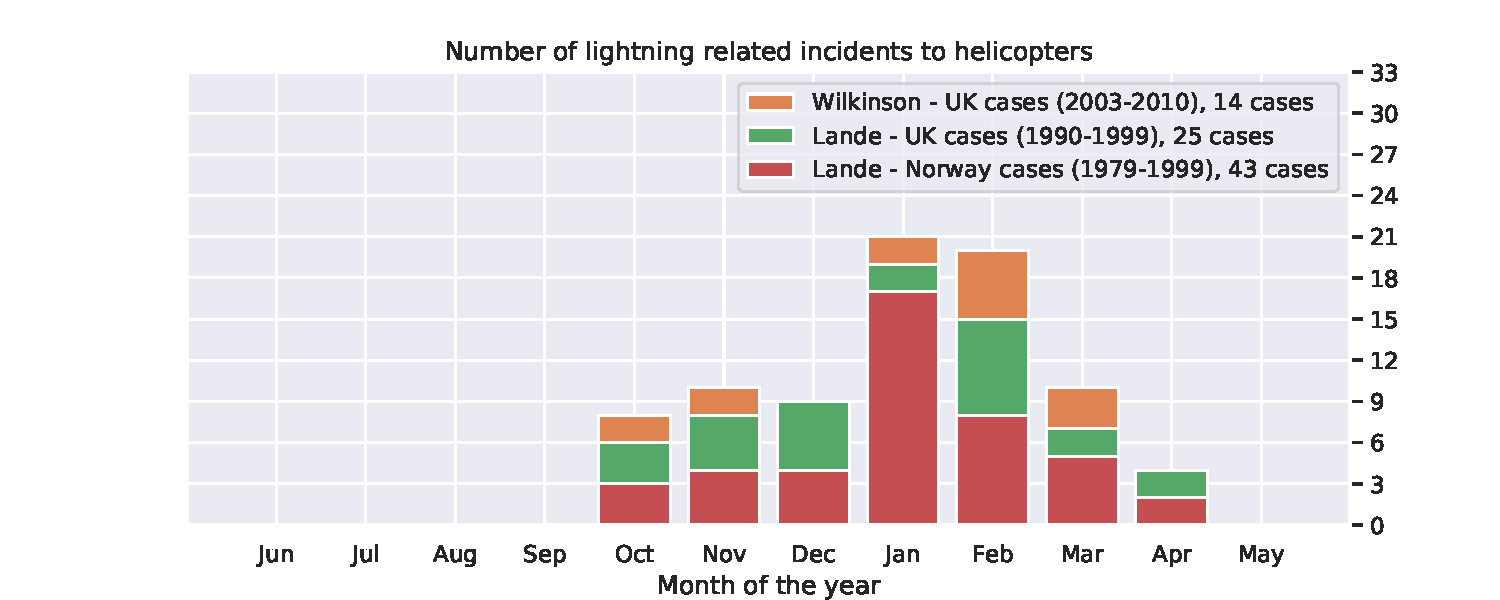
\includegraphics[width=\textwidth]{Figures/yearlydistribution_withoutmine.pdf}
    \caption{Seasonal variation of helicopter cases, showing no cases in May to September. Data is produced from \cite{lande1999} and \cite{wilkinson2013}. Legend notes time-periods and amount of cases in each study.}
    \label{fig:landewilk}
\end{figure}

The study of \acrshort{htl} had its peak around the turn of the century, due to two helicopter incidents related to lightning (1995 and 2002). The 1995 incident was a non-fatal incident. A lightning strike destroyed the main rotor of the helicopter, forcing the pilot to perform a landing in the ocean (\cite{smart1997}). The 2002 incident resulted in eleven fatalities and is believed to have been caused by internal damage to the helicopter's main rotor back in 1997. The initial inspection of the rotor did not uncover any damage, causing the helicopter to be cleared for flight. This initial structural damage later resulted in failure of the main rotor, leading to the crash in 2002 (\cite{smart2005}). These events resulted in practical guidelines to helicopter pilots based on data from earlier incidents (\cite{lande1999}, \cite{hardwick1999}). Furthermore, the UK Met Office added numerical simulation and forecasting to these guidelines, with the introduction of \acrfull{hti}. This provided a more robust warning for helicopter pilots (\cite{wilkinson2013}). Since then, general \acrfull{nwp} forecasts have improved and continue to improve due to better  physical understanding, more and higher quality observations, and increase in available computational power. This thesis aims to improve upon the understanding of the \acrshort{htl} phenomenon by using state-of-the-art model products as described in Section \ref{sec:models}.

The author makes use of a novel dataset from Avinor containing reported incidents of both \acrshort{htl} and a similar phenomenon: \acrfull{fwtl}. \acrshort{fwtl} is triggered lightning involving planes and rockets, where the wings are fixed. \acrshort{fwtl}, unlike \acrshort{htl}, is of less danger to both personnel and materials. Fixed wing aircraft are generally hit in the main body. Fuel and vital electronics are also better protected in fixed wing aircraft (\cite{petrov2012}). Helicopters are mainly hit through the rotor into the main body (\cite{lande1999}). Despite this difference in actual risk, both incidents are associated with non-negligible risk, and require thorough inspection of the aircraft after the fact.

To investigate atmospheric conditions during \acrshort{htl} and \acrshort{fwtl} incidents, the \acrfull{era5} data set is utilized. Also used for this purpose is the operational \acrfull{meps}\footnote{\acrfull{metcoop}}. 

These are the research questions this thesis attempts to answer:
\begin{itemize}	
    \item Are there still cases of \acrlong{htl} in Norway?
    \item What meteorological phenomena are present during triggered lightning incidents?
    \item In what ways can the \acrshort{htl} forecast be improved?
\end{itemize}

The goal is to improve and strengthen the confidence in the current operational \acrshort{htl} forecast. Also under investigation is an error found in the algorithm used to produce the operational forecast where the accumulated precipitation, and not the intended hourly precipitation, was used in the operational forecast. This lead to a potential over-estimation of risk related to offshore flights.
